\documentclass{article}

\usepackage{amsmath, amssymb}
\usepackage{float}
\usepackage{graphicx}
\usepackage{subcaption}
\usepackage{color}

\usepackage{listings}


\definecolor{dkgreen}{rgb}{0,0.6,0}
\definecolor{gray}{rgb}{0.5,0.5,0.5}
\definecolor{mauve}{rgb}{0.58,0,0.82}

\lstset{frame=tb,
  language=python,
  aboveskip=3mm,
  belowskip=3mm,
  showstringspaces=false,
  columns=flexible,
  basicstyle={\small\ttfamily},
  numberstyle=\color{gray},
  keywordstyle=\color{blue},
  commentstyle=\color{dkgreen},
  stringstyle=\color{mauve},
  breaklines=true,
  breakatwhitespace=true,
  tabsize=3,
}
%

\addtolength{\topmargin}{-.875in}
\addtolength{\textheight}{1.75in}


\title{Project report - Week 3}

\begin{document}
	\maketitle
	\section{Introduction}
	
	    While working on flower recognition we hit the glass ceiling. We no longer were able to improve our network that is why we decided to use transfer learning.
	    
	    The idea behind it is taking advantage of pre-trained neural network that have been developed by professionals.
        Instead of building a network from scratch, we just change the last layer in high-performance neural network.
        
        In our case we used MobileNet, which is a light neural network trained on ImageNet data set. ImageNet has 1000 classes of different objects, but we can apply it to our problem, by changing and training last layer. It is important not to train the MobileNet part of network to not mess it up.
	    
	    Implementation of transfer learning is easy and training time is low, that is because we train only the last layer of our model.
	    
	\section{Results}
			\begin{figure}[H]
				\centering
				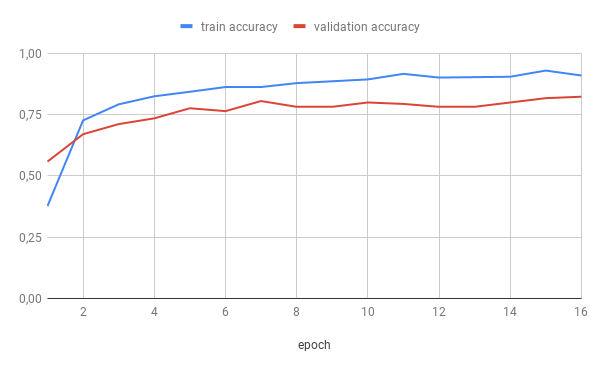
\includegraphics[width = 12cm]{chart_accurcy.png}
				\caption{Results of Transfer Learning over 16 epochs.}		
			\end{figure}
			\begin{figure}[H]
				\centering
				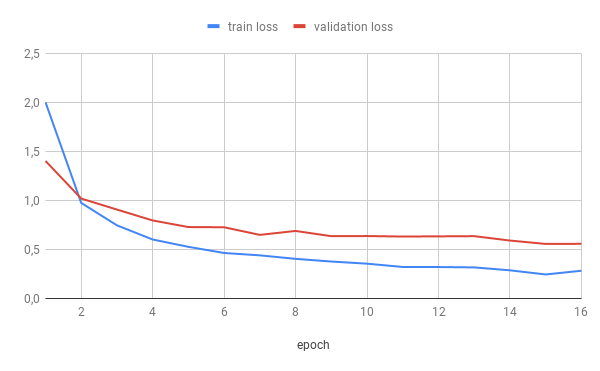
\includegraphics[width = 12cm]{chart_loss.png}
				\caption{Results of Transfer Learning over 16 epochs.}		
			\end{figure}
			The input image has to have size of 128x128, because the first part of your network is MobileNet, which require such an image.
			
			Based on the charts we can see that the network archive about 80\% accuracy after 10 epochs.
	
	\section{Summary}
		Use of transfer learning allowed us to train fast high-performance neural network. What is more we can solve many similar problems using this technique.
\end{document}